% Options for packages loaded elsewhere
\PassOptionsToPackage{unicode}{hyperref}
\PassOptionsToPackage{hyphens}{url}
\documentclass[
]{book}
\usepackage{xcolor}
\usepackage{amsmath,amssymb}
\setcounter{secnumdepth}{5}
\usepackage{iftex}
\ifPDFTeX
  \usepackage[T1]{fontenc}
  \usepackage[utf8]{inputenc}
  \usepackage{textcomp} % provide euro and other symbols
\else % if luatex or xetex
  \usepackage{unicode-math} % this also loads fontspec
  \defaultfontfeatures{Scale=MatchLowercase}
  \defaultfontfeatures[\rmfamily]{Ligatures=TeX,Scale=1}
\fi
\usepackage{lmodern}
\ifPDFTeX\else
  % xetex/luatex font selection
\fi
% Use upquote if available, for straight quotes in verbatim environments
\IfFileExists{upquote.sty}{\usepackage{upquote}}{}
\IfFileExists{microtype.sty}{% use microtype if available
  \usepackage[]{microtype}
  \UseMicrotypeSet[protrusion]{basicmath} % disable protrusion for tt fonts
}{}
\makeatletter
\@ifundefined{KOMAClassName}{% if non-KOMA class
  \IfFileExists{parskip.sty}{%
    \usepackage{parskip}
  }{% else
    \setlength{\parindent}{0pt}
    \setlength{\parskip}{6pt plus 2pt minus 1pt}}
}{% if KOMA class
  \KOMAoptions{parskip=half}}
\makeatother
\usepackage{longtable,booktabs,array}
\usepackage{calc} % for calculating minipage widths
% Correct order of tables after \paragraph or \subparagraph
\usepackage{etoolbox}
\makeatletter
\patchcmd\longtable{\par}{\if@noskipsec\mbox{}\fi\par}{}{}
\makeatother
% Allow footnotes in longtable head/foot
\IfFileExists{footnotehyper.sty}{\usepackage{footnotehyper}}{\usepackage{footnote}}
\makesavenoteenv{longtable}
\usepackage{graphicx}
\makeatletter
\newsavebox\pandoc@box
\newcommand*\pandocbounded[1]{% scales image to fit in text height/width
  \sbox\pandoc@box{#1}%
  \Gscale@div\@tempa{\textheight}{\dimexpr\ht\pandoc@box+\dp\pandoc@box\relax}%
  \Gscale@div\@tempb{\linewidth}{\wd\pandoc@box}%
  \ifdim\@tempb\p@<\@tempa\p@\let\@tempa\@tempb\fi% select the smaller of both
  \ifdim\@tempa\p@<\p@\scalebox{\@tempa}{\usebox\pandoc@box}%
  \else\usebox{\pandoc@box}%
  \fi%
}
% Set default figure placement to htbp
\def\fps@figure{htbp}
\makeatother
\setlength{\emergencystretch}{3em} % prevent overfull lines
\providecommand{\tightlist}{%
  \setlength{\itemsep}{0pt}\setlength{\parskip}{0pt}}
\usepackage[]{natbib}
\bibliographystyle{plainnat}
\usepackage{booktabs}
\usepackage{bookmark}
\IfFileExists{xurl.sty}{\usepackage{xurl}}{} % add URL line breaks if available
\urlstyle{same}
\hypersetup{
  pdftitle={Statistics For Science Extension},
  pdfauthor={Michael Dear},
  hidelinks,
  pdfcreator={LaTeX via pandoc}}

\title{Statistics For Science Extension}
\author{Michael Dear}
\date{2026-03-13}

\begin{document}
\maketitle

{
\setcounter{tocdepth}{1}
\tableofcontents
}
\chapter{Introduction}\label{introduction}

\begin{quote}
\textbf{Learning Objectives}\\
To define statistics and its purpose\\
To review the process and design of scientific studies\\
To understand the difference between populations and samples\\
To understand the difference between descriptive and inferential statistics
\end{quote}

These notes are a practical introduction to statistics for students of the NSW Science Extension course. The emphasis is on learning through examples and problem-solving.

\section{What Is Statistics and What Does It Do?}\label{what-is-statistics-and-what-does-it-do}

There is no one simple definition for what statistics is and what it does.

``Statistics uses samples to explain and predict''

``Statistics is a set of techniques for collecting and analysing data''

``Statistics tells the story of the population being studied''

However, it can be said that statistics is fundamental to all stages of scientific research.

\section{Examples of Statistical Problems}\label{examples-of-statistical-problems}

Most scientific research questions will rely heavily on statistical techniques:

\begin{itemize}
\tightlist
\item
  What is the average girth (circumference) of trees in a forest?
\item
  What is the rate of decline in seabird populations in Australian coastal waters?
\item
  Does a new vaccine reduce the number of deaths from influenza?
\item
  Predict the rise in temperature by 2050 in different regions of Australia.
\end{itemize}

\section{A More Detailed Example}\label{a-more-detailed-example}

Forestry scientists would like to know the average girth (circumference) of trees in a forest. There are too many trees to measure them all, so they plan to take a random sample of 200 trees. They need to use statistics to determine the size and structure of the sample. After collecting the data, they complete a statistical analysis to estimate that, to a high level of confidence, the average tree girth is between 175cm and 225cm. They then write a report using statistical tables and plots to communicate their results.

\section{Scientific Studies}\label{scientific-studies}

A scientific study has the following steps:

\begin{itemize}
\tightlist
\item
  Research question(s)
\item
  Study design - experimental or observational?
\item
  Data collection
\item
  Data analysis
\item
  Report
\end{itemize}

\section{Study Design}\label{study-design}

There are two basic types of scientific study:

\begin{quote}
\textbf{Observational study} - variables are not controlled e.g.~the health records of 1000 people who had taken Drug X were reviewed to determine the side effects.
\end{quote}

\begin{quote}
\textbf{Experimental study} - variables are controlled e.g.~Plots A and B are next to each other. Plot A receives fertiliser and Plot B receives none.
\end{quote}

Observational studies can show \emph{associations} between variables, but experimental studies can show \emph{causal} relationships.

\begin{quote}
Observational study \(\rightarrow\) association - ``A varies as B varies''\\
Experimental study \(\rightarrow\) causation - ``A causes B''
\end{quote}

\section{Population and Sample}\label{population-and-sample}

\begin{quote}
\textbf{Population} - all members of the group being studied e.g.~all the Magpies in NSW. Population values are called \textbf{parameters}.
\end{quote}

\begin{quote}
\textbf{Sample} - a subset of the population being studied e.g.~1000 magpies chosen at random locations across NSW. Sample values are called \textbf{statistics}.
\end{quote}

\section{Symbols For Common Values}\label{symbols-for-common-values}

\begin{longtable}[]{@{}lll@{}}
\toprule\noalign{}
Value & Population Parameter & Sample Statistic \\
\midrule\noalign{}
\endhead
\bottomrule\noalign{}
\endlastfoot
Mean & \(\mu\) & \(\bar{x}\) \\
Standard Deviation & \(\sigma\) & \(s\) \\
Proportion & \(p\) & \(\hat{p}\) \\
\end{longtable}

\section{Descriptive and Inferential Statistics}\label{descriptive-and-inferential-statistics}

\begin{quote}
\textbf{Descriptive statistics} describe data e.g.~mean, median, standard deviation of a data set.
\end{quote}

\begin{quote}
\textbf{Inferential statistics} estimate population parameters from a sample.
\end{quote}

Statistical analysis usually begins with descriptive statistics, then moves on to inferential statistics.

\begin{center}\rule{0.5\linewidth}{0.5pt}\end{center}

\section{Extension - Spreadsheets and Statistical Computing Languages}\label{extension---spreadsheets-and-statistical-computing-languages}

Spreadsheets are handy for recording and exploring small data sets. However, the capabilities of spreadsheets for statistical analysis are limited. Larger projects are best completed using a statistical computing language such as R. Analyses completed using computer coding have many advantages, such as

\begin{itemize}
\tightlist
\item
  the ability to handle very large data sets
\item
  a greater variety of plots
\item
  greater control over plot and data output
\item
  the availability of sophisticated modelling techniques
\item
  a coding script becomes a reproducible record of the steps completed during the project
\end{itemize}

The disadvantage of coding is the time taken to learn a language, although there are numerous training resources and forums available for free on the internet.

These notes, including plots, tables, and most diagrams, were created using the R statistical computing language.

\begin{center}\rule{0.5\linewidth}{0.5pt}\end{center}

\section{Activity}\label{activity}

Write definitions for each term:

\begin{itemize}
\tightlist
\item
  Population
\item
  Parameter
\item
  Sample
\item
  Statistic
\item
  Experimental study
\item
  Causation
\item
  Observational study
\item
  Association
\item
  Descriptive statistics
\item
  Inferential statistics
\end{itemize}

\chapter{Data Concepts}\label{data_concepts}

\begin{quote}
\textbf{Learning Objectives}\\
To uderstand the basic types of data\\
To understand how data is structured for statistical analysis\\
To determine the amount of data required for a scientific study\\
To investigate methods of data collection\\
To distinguish between primary and secondary sources\\
To review some secondary sources of scientific data\\
To learn the steps in preparing data for statistical analysis
\end{quote}

\section{Types of Data}\label{types-of-data}

\begin{figure}
\centering
\pandocbounded{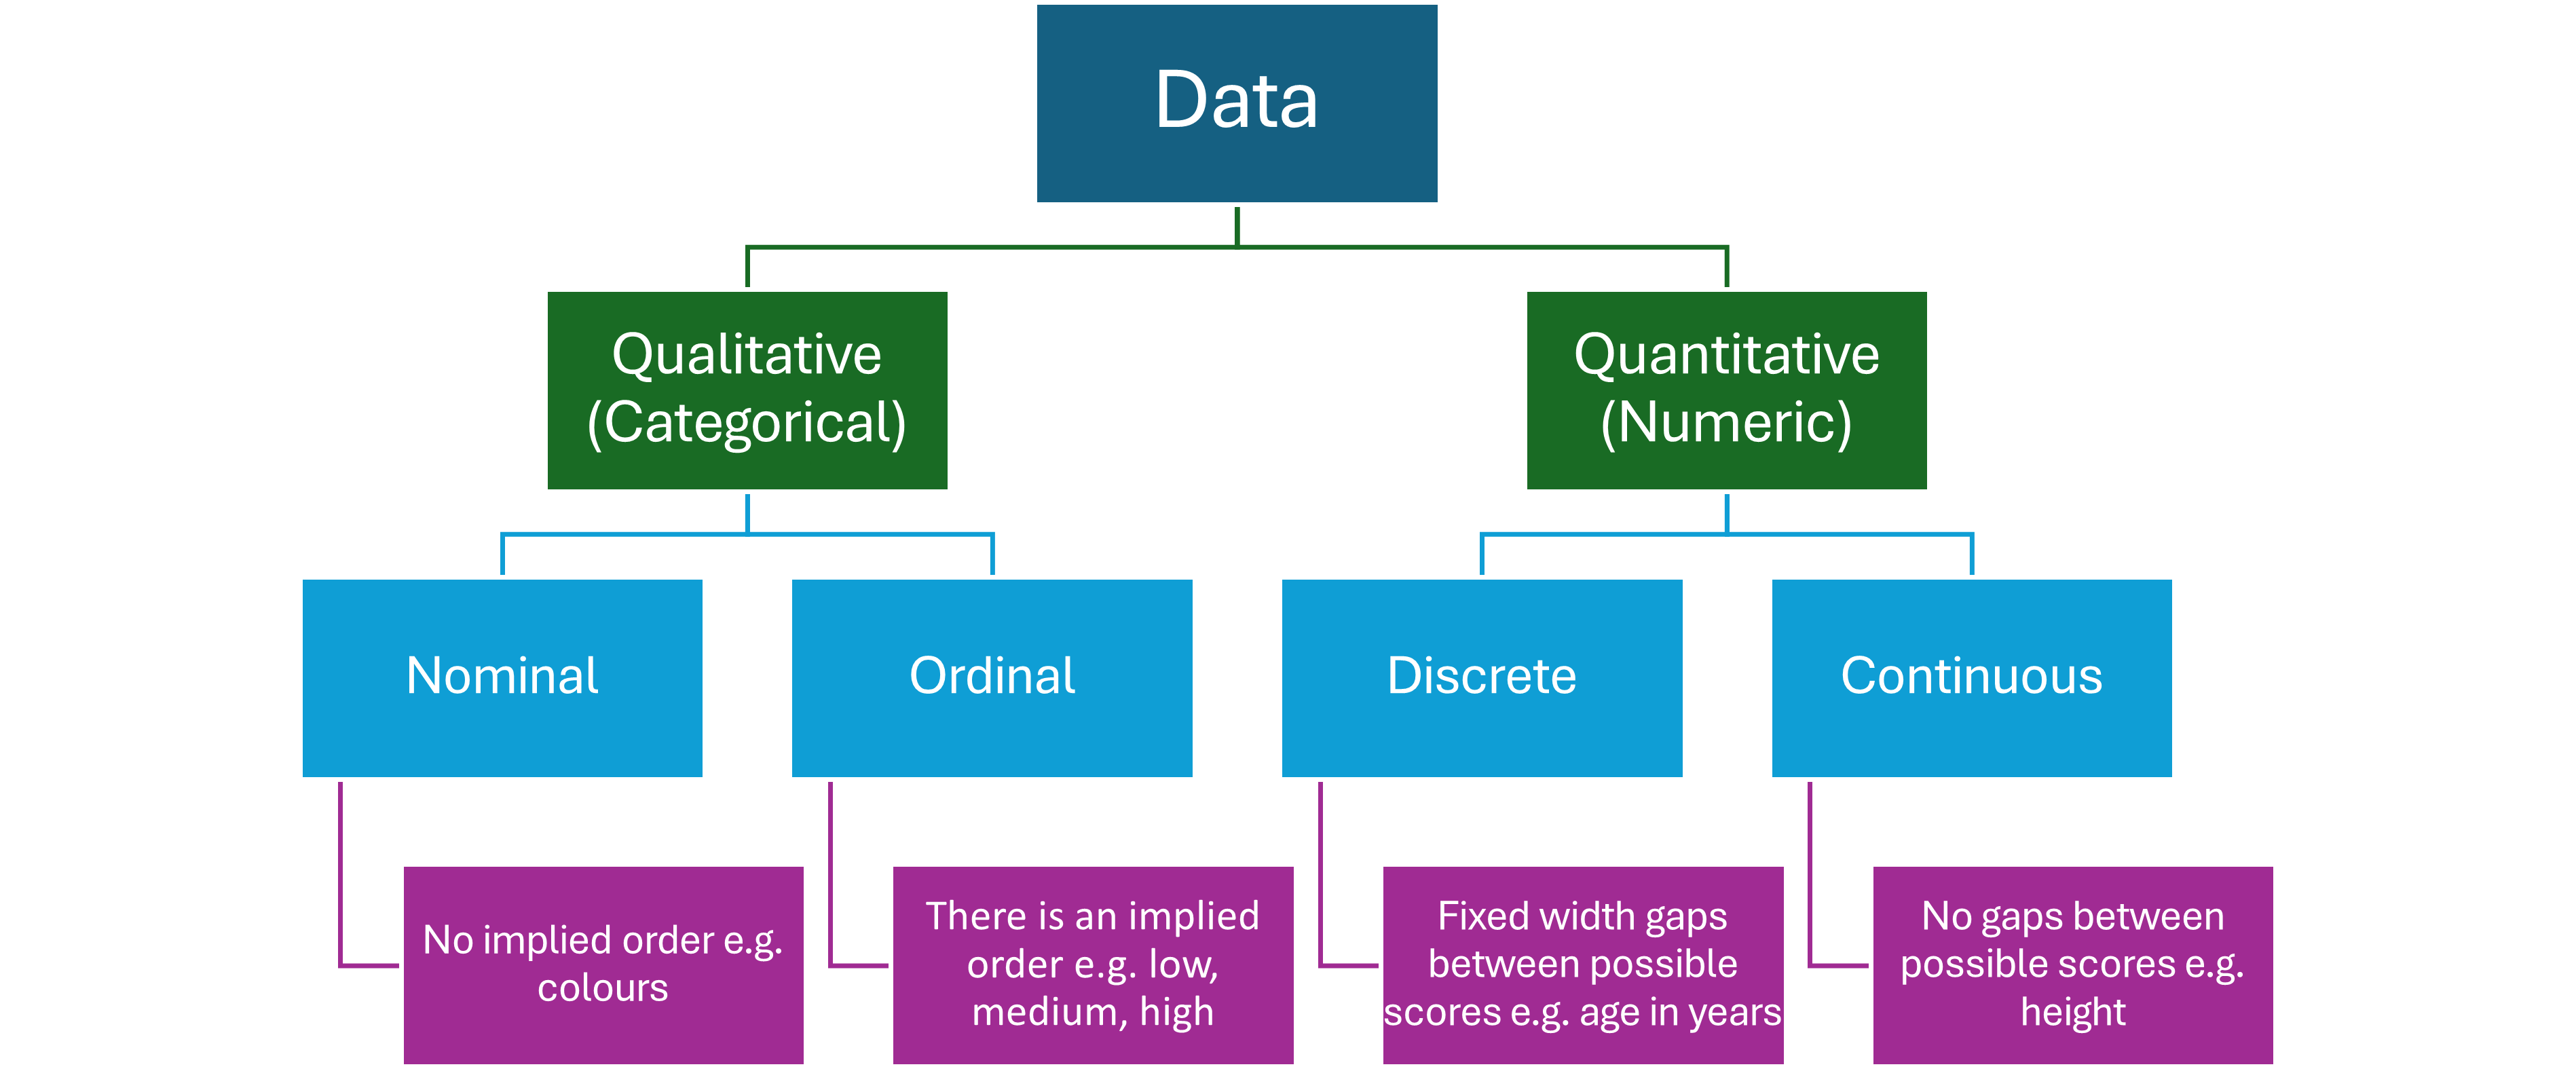
\includegraphics[keepaspectratio]{./resources/img/types_of_data.png}}
\caption{The basic types of data.}
\end{figure}

\begin{quote}
\emph{Count data} is quantitative discrete data in which the number of occurrences of something are recorded e.g.~the number of birds in migratory flocks.
\end{quote}

\section{The Structure of Data}\label{the-structure-of-data}

Data should be structured using tables in which

\begin{itemize}
\tightlist
\item
  each column represents a variable
\item
  the values in each column are the same type and the same unit
\item
  the first row contains the names of the variables without any spaces
\end{itemize}

The data in each row represents a single \emph{observation} of the variables. Observations are often called \emph{records} or \emph{cases}, depending on the context of the study. Similarly, columns are often called \emph{attributes}, \emph{features} or \emph{fields}.

\subsection{File Formats For Data Storage and Exchange}\label{file-formats-for-data-storage-and-exchange}

The most common format for storing and exchanging data for statistical analysis is \emph{comma separated format} (CSV). CSV is a plain text file with fields separated by commas. Numeric data is unquoted and text data is surrounded by quotation marks. CSV files usually have the extension ``.csv''.

The following is an example of CSV file contents. The first row is the column headers, and the remaining rows are observations.

\begin{verbatim}
"Sepal.Length","Sepal.Width","Petal.Length","Petal.Width","Species"
5.1,3.5,1.4,0.2,"setosa"
4.9,3,1.4,0.2,"setosa"
4.7,3.2,1.3,0.2,"setosa"
\end{verbatim}

\subsection{Activity}\label{activity-1}

\begin{enumerate}
\def\labelenumi{\arabic{enumi}.}
\tightlist
\item
  List the variables and the type of data they represent for the following data set.
\item
  Write down one observation from the table.
\end{enumerate}

\begin{verbatim}
 Sepal.Length Sepal.Width Petal.Length Petal.Width    Species
          5.9         3.0          5.1         1.8  virginica
          5.5         4.2          1.4         0.2     setosa
          7.1         3.0          5.9         2.1  virginica
          6.3         2.8          5.1         1.5  virginica
          5.8         2.6          4.0         1.2 versicolor
          5.8         4.0          1.2         0.2     setosa
\end{verbatim}

\section{Collecting Data}\label{collecting-data}

Data sources can be classified as either \emph{primary} or \emph{secondary}.

\begin{quote}
\textbf{Primary Source Data} is collected by the researcher through first-hand surveys.\\
\textbf{Secondary Source Data} is collected from existing data repositories.
\end{quote}

\subsection{Sample Size - How Much Data Is Enough?}\label{sample-size---how-much-data-is-enough}

Estimating the sample size for a research project is important because

\begin{itemize}
\tightlist
\item
  sample size needs to be large enough to detect the expected effect if it's present
\item
  a sample that is too large is wasteful of resources or could be unethical
\item
  the study might not be feasible if a large sample size is required.
\end{itemize}

Estimating sample size depends on

\begin{itemize}
\tightlist
\item
  the objective(s) of the research
\item
  the type of statistical tests or modelling that will be applied
\item
  the type of study design e.g.~experimental versus observational studies
\item
  if the target outcome is a rare case
\end{itemize}

Sample size can be estimated using software tools or, for situations where less scientific rigor is required, by ``rules of thumb''.

\begin{center}\rule{0.5\linewidth}{0.5pt}\end{center}

\subsection{Extension}\label{extension}

You might come across them in your research when estimating the sample size required for your project.

\begin{quote}
\textbf{Definitions}
\textbf{Type I Error} - rejecting a true null hypothesis (false positive - accepting there is a significant effect when there isn't one)\\
\textbf{Type II Error} - not rejecting a false null hypothesis (false negative - missing a significant effect when there is one)\\
\textbf{Power} - the ability of a statistical test to detect an effect given that the effect exists. Formal definition: \(\text{Power} = 1 - \text{P(Type II Error)}\)
\end{quote}

We will come back to hypothesis testing in a later lesson.

\begin{center}\rule{0.5\linewidth}{0.5pt}\end{center}

\subsection{Large Data Sets}\label{large-data-sets}

Large data sets have become commonplace since the advent of the internet and increasingly powerful computers. While these data sets provide the ability to work with very large samples, they introduce the problem of ``information overload''. Too much data can be as big a problem as too little data!

To overcome some of the problems associated with large data sets, they are increasingly available online along with the ability to process the data using cloud computing. This makes the task of working with large data sets more achievable for individuals and smaller institutions.

\subsection{Activity - Online Data Repositories}\label{activity---online-data-repositories}

Explore the following data repositories and complete the table.

\begin{longtable}[]{@{}
  >{\raggedright\arraybackslash}p{(\linewidth - 6\tabcolsep) * \real{0.2083}}
  >{\raggedright\arraybackslash}p{(\linewidth - 6\tabcolsep) * \real{0.1875}}
  >{\raggedright\arraybackslash}p{(\linewidth - 6\tabcolsep) * \real{0.1458}}
  >{\raggedright\arraybackslash}p{(\linewidth - 6\tabcolsep) * \real{0.4583}}@{}}
\toprule\noalign{}
\begin{minipage}[b]{\linewidth}\raggedright
Repository
\end{minipage} & \begin{minipage}[b]{\linewidth}\raggedright
Main Uses
\end{minipage} & \begin{minipage}[b]{\linewidth}\raggedright
Formats
\end{minipage} & \begin{minipage}[b]{\linewidth}\raggedright
Cloud Processing (y/n)
\end{minipage} \\
\midrule\noalign{}
\endhead
\bottomrule\noalign{}
\endlastfoot
\href{https://www.abs.gov.au/}{ABS} & & & \\
\href{https://data.gov.au/}{data.gov.au} & & & \\
\href{https://www.seed.nsw.gov.au/}{SEED NSW} & & & \\
\href{https://www.ga.gov.au/scientific-topics/dea}{Digital Earth Australia} & & & \\
\href{https://www.ala.org.au/}{Atlas of Living Australia} & & & \\
\end{longtable}

\section{Data Cleaning}\label{data-cleaning}

Most data needs preparation or ``cleaning'' before statistical analysis can begin.

There is an expression that says ``10 percent inspiration, 90 percent perspiration''. In the case of statistics, preparing data for analysis is often the ``90 percent perspiration''! Most real-world data sets will need a lot of cleaning before they are suitable for use in a research project.

Some of the issues that need to be checked and remedied are

\begin{itemize}
\tightlist
\item
  missing values, often labelled as \textbf{NA}, but might just be blank - impute, drop, or ignore?
\item
  incorrect number formats e.g.~differing numbers of decimal places, missing decimal points: 1.02, 1.15, 103, 1.96
\item
  units included in quantitative columns e.g.~9.1, 3.2, 5.8mm, 6.7
\item
  Not the correct number of rows e.g.~your data set should have 1000 rows, but it only has 100 when you open it
\item
  duplicate categories in qualitative variables e.g.~dog, cat, cat, dogs, cats
\item
  dates and times are not recognised correctly by the software
\item
  outliers
\item
  duplicate records
\item
  removing irrelevant variables; finding the relevant ones amongst hundreds
\item
  variables that have only one value or are empty
\item
  column names that contain characters not permitted in some computing languages e.g.~\%, \#, \$
\item
  columns that have no name
\item
  metadata added at the beginning or end of data tables exported from secondary sources - always check the end of the data for unwanted additions!
\item
  empty rows, cells, merged cells in spreadsheets :(
\end{itemize}

\ldots{} and the list goes on.

\begin{quote}
\textbf{Tip}\\
For a small project where you are working alone or in a small team, avoid most of these problems by developing a thorough plan and keeping accurate records. Do not change your methods once you have started recording data.
\end{quote}

\subsection{Activity}\label{activity-2}

Open the \href{resources/datasets/messy_data.csv}{messy\_data.csv} data set in a spreadsheet. This data represents observations from a national wildlife database for a study area. Find any issues with the data and decide what should be done to prepare the data for analysis.

\chapter{Further Reading}\label{further_reading}

\section{Books}\label{books}

\section{Websites}\label{websites}

\href{https://www.abs.gov.au/statistics/understanding-statistics/statistical-terms-and-concepts}{\textbf{Australian Bureau of Statistics ``Statistical Terms and Concepts''}} : A comprehensive glossary pf statistical terms. Click the terms for detailed explanations.

\bibliography{book.bib,packages.bib}

\end{document}
